\documentclass[uplatex, twocolumn, dvipdfmx, 10pt]{jsarticle}
\和暦
\usepackage[top=25truemm,bottom=25truemm,left=25truemm,right=25truemm]{geometry}
\usepackage[dvipdfmx]{graphicx}
\usepackage{color}
\setlength{\columnsep}{3zw}

\title{ブロックチェーンプログラムの実装}
\author{744069\ 池田 敬祐}
\date{\today}

\begin{document}

\twocolumn[
  \maketitle
  \begin{abstract}
  \ \ \ 不完全なブロックチェーンプログラムを自らの手で完成させる。完成させたプログラムを用いてハッシュ値の基準(difficultyBits)を変更させた時の実行時間の変動を計測する。
  結果よりハッシュ値の基準(difficultyBits)とプログラムを実行するマシンスペックが実行時間に影響を与えていることがわかった。以上の工程を通じてブロックチェーンの仕組みを理解した。
  \\
  \end{abstract}
]

\section{はじめに}
本課題では講義中に配布された不完全なブロックチェーンプログラムを完成させることを目標とする。
その後、ハッシュ値の基準(difficultyBits)を変更させた時に完成させたプログラムの実行時間がどのように変動するかを計測し、ブロックチェーン、Javaによる並列プログラミングへの理解を深めることを目的とする。

\section{実装内容の説明}
配布されたブロックチェーンプログラムの一部である「MiningNode.java」の「run()」「broadcastBlock()」「receiveMiner()」「createBlock()」「validateBlock()」「addBlockToChain()」の6つのメソッドの実装を行った。
また、実装を行うと同時にブロックチェーンプログラム全体のリファクタリングも行った。
\begin{description}
  \item[(1)]「run()」
  \\\ \ \ 「MiningNode.java」のメインメソッド。ハッシュ値のマイニングや、Block生成、他プロセスとの通信、ブロックチェーンへのBlock追加などを行う。
  メソッドではプロセスが0(最初のプロセス)の時とそれ以外の時で処理がやや異なる。
  プロセスが0の時、ブロックチェーンの先頭のBlockを生成したのち本メソッドの機能を満たす記述を行った。
  それ以外の時、他プロセスとの通信が正確に行われる必要があった。最初にループ文を用いて通信が行われるまで次の処理に進まないように制御することで機能を満たした。
  \item[(2)]「broadcastBlock()」
  \\\ \ \ 他プロセスにBlockを送信するメソッドである。実装済みのメソッドである「broadcastMiner()」を参考に実装を行った。
  \item[(3)]「receiveMiner()」
  \\\ \ \ 追加したメソッド。他プロセスからMinerを受信するためのメソッドである。実装済みのメソッドである「receiveBlock()」を参考に実装を行った。
  \item[(4)]「createBlock()」
  \\\ \ \ 新たなBlockを生成するメソッド。引数として入力されたResultなどの情報を元にBlockクラスをインスタンス化することで機能を満たしている。
  \item[(5)]「validateBlock()」
  \\\ \ \ Blockのハッシュ値が基準を満たしているかチェックするメソッド。実装済みのメソッドである「checkHashValues()」を参考に実装を行った。
  \item[(6)]「addBlockToChain()」
  \\\ \ \ 新しいBlockをブロックチェーンの末端に接続する。プログラムではブロックチェーンをBlockのArrayListとして実装されている。
  本メソッドではArrayListの「add()」メソッドを呼び出し、引数として入力された新しいBlockを追加することで機能を満たしている。
\end{description}

\section{実行方法}
ターミナルを開き、プログラムが存在するディレクトリに移動する。そこで、「sh javac.sh *.java」を入力し、プログラムをまとめてコンパイルする。
次に「sh java.sh Simulator -c MiningNode」を入力して実行をする。この際に「-p」オプションでプロセスを指定したり、「-t」オプションで実行時間の計測を行うことが可能である。
例えば「sh java.sh Simulator -c MiningNode -p 3 -t」と入力することでプロセス数を3として実行時間を計測しつつ実行が可能である。

\section{計測方法}
今回の計測ではプロセス数を3に固定する。ハッシュ値の基準(difficultyBits)を10から20の範囲で変更していき、それぞれの場合での実行時間を2つの環境で計測する。
計測は以下の2つの環境で行った。
\begin{description}
  \item[(1)]計測環境①「MacBook Retina 12 [2017]」
  \\・プロセッサ:Intel Core i5 1.3GHz 
  \\・メモリ:8GB 1,866MHz LPDDR3
  \\・PCIe-based onboard flash storage:512GB
  \\・Intel HD Graphics 615
  \item[(2)]計測環境②「Mac mini」
  \\・プロセッサ:Intel Core i7 2.6GHz
  \\・メモリ:8GB
  \\・Internal Solid State Drive:500GB 
  \\・Intel HD Graphics 4000 (1024MB)
\end{description}

\section{計測結果}
計測結果として表1のように値が得られた。表1の計測結果の単位は[msec]であり、小数点以下は切り上げている。
なお、計測環境①を①、計測環境②を②と省略して表記している。また、時間の関係により、計測が間に合わなかったものは「-」と表記している。
表1をグラフにしたものが図1である。赤色の線が計測環境①の平均、青色の線が計測結果②の平均、緑色の線が総合平均を表している。縦軸を時間[msec]、横軸をdifficultyBitsとする。

\section{考察}
計測結果より、difficultyBitsが大きいほど、実行時間が長くなる傾向にあることが分かる。しかし、これは傾向であり、絶対的な規則でないこともわかった。
例えば表1の計測環境①のdifficultyBitsが13と14の時を比較する。difficultyBitsが13の時は230464[msec]であるのに対し、difficultyBitsが14の時は168849[msec]となっており、値が減少していた。
このような結果が出た理由として、ブロックチェーンが行うマイニングが絶対的な処理でなく、確率的な処理であることがあげられる。
difficultyBitsとはあくまでマイニングが成功する度合いを示したものであるため、今回のように低確率で減少することもあるのだと私は結論づけた。
以上の考察は表1にある、同じ環境下で同じdifficultyBitsであるにも関わらず、値が大きく異なるケースにも言うことができる。
実行時間に影響を与えたのはdifficultyBitsだけではない。プログラムを実行するマシンスペックも大きな影響を与えていると言える。
その根拠としてdifficultyBitsが20の時の計測環境①と計測環境②の結果を比較する。計測環境②の結果に対して計測環境①の方は2倍近い値が出ている。
これは上述した確率が左右していることもあるが、それにしても差分が大きい。これら2つの違いとして他にあげられるのはマシンスペックの違いである。
計測環境①と計測環境②のマシンスペックの違いは既に前章の計測方法で述べているが計測環境②の方がマシンスペックは良く、そのため計算速度に差がでたのではないかと結論づけた。

\section{まとめ}
以上の結果・考察より、ブロックチェーンの実行時間にはハッシュ値の基準(difficultyBits)とプログラムを実行するマシンスペックが影響を与えていることがわかった。
今回はプロセス数を3、ブロック数が5と固定して計測したが、本来のブロックチェーンではプロセス数、ブロック数共に莫大な数が必要となる。これらの値を変動した時の実行時間の変動について調査することも有意義であると私は考える。

\begin{table*}[htb]
  \begin{center}
    \caption{実行時間の変動の表}
    \begin{tabular}{|r|r|r|r|r||r|r|r|} \hline
      difficultyBits & ①1回目 & ①2回目 & ②1回目 & ②2回目 & ①平均 & ②平均 & 総合平均\\ \hline \hline
      20 & 16091191 & - & 8585046 & - & 16091191 & 8585046 & 12338119\\
      19 & - & - & 3859165 & - & - & 3859165 & 3859165\\
      18 & 4243843 & - & 1916662 & - & 4243843 & 1916662 & 3080253 \\
      17 & 1264988 & - & 2215404 & 3047552 & 1264988 & 2631478 & 1948233\\
      16 & 1102612 & 1448993 & 781351 & 466263 & 1275803 & 623807 & 949805\\
      15 & 954947 & 257300 & 536190 & 573253 & 606124 & 554722 & 580423\\
      14 & 168849 & 221047 & 147541 & 128549 & 194948 & 138045 & 166497\\
      13 & 230464 & 228480 & 110492 & 62343 & 229472 & 86418 & 157945\\
      12 & 230022 & 55691 & 62269 & 167864 & 142857 & 115067 & 128962\\
      11 & 46641 & 44266 & 45270 & 32227 & 45454 & 38749 & 42101\\
      10 & 7091 & 9104 & 11137 & 22180 & 8098 & 33317 & 20707\\ \hline
    \end{tabular}
  \end{center}
\end{table*}

\begin{figure*}
  \begin{center}
    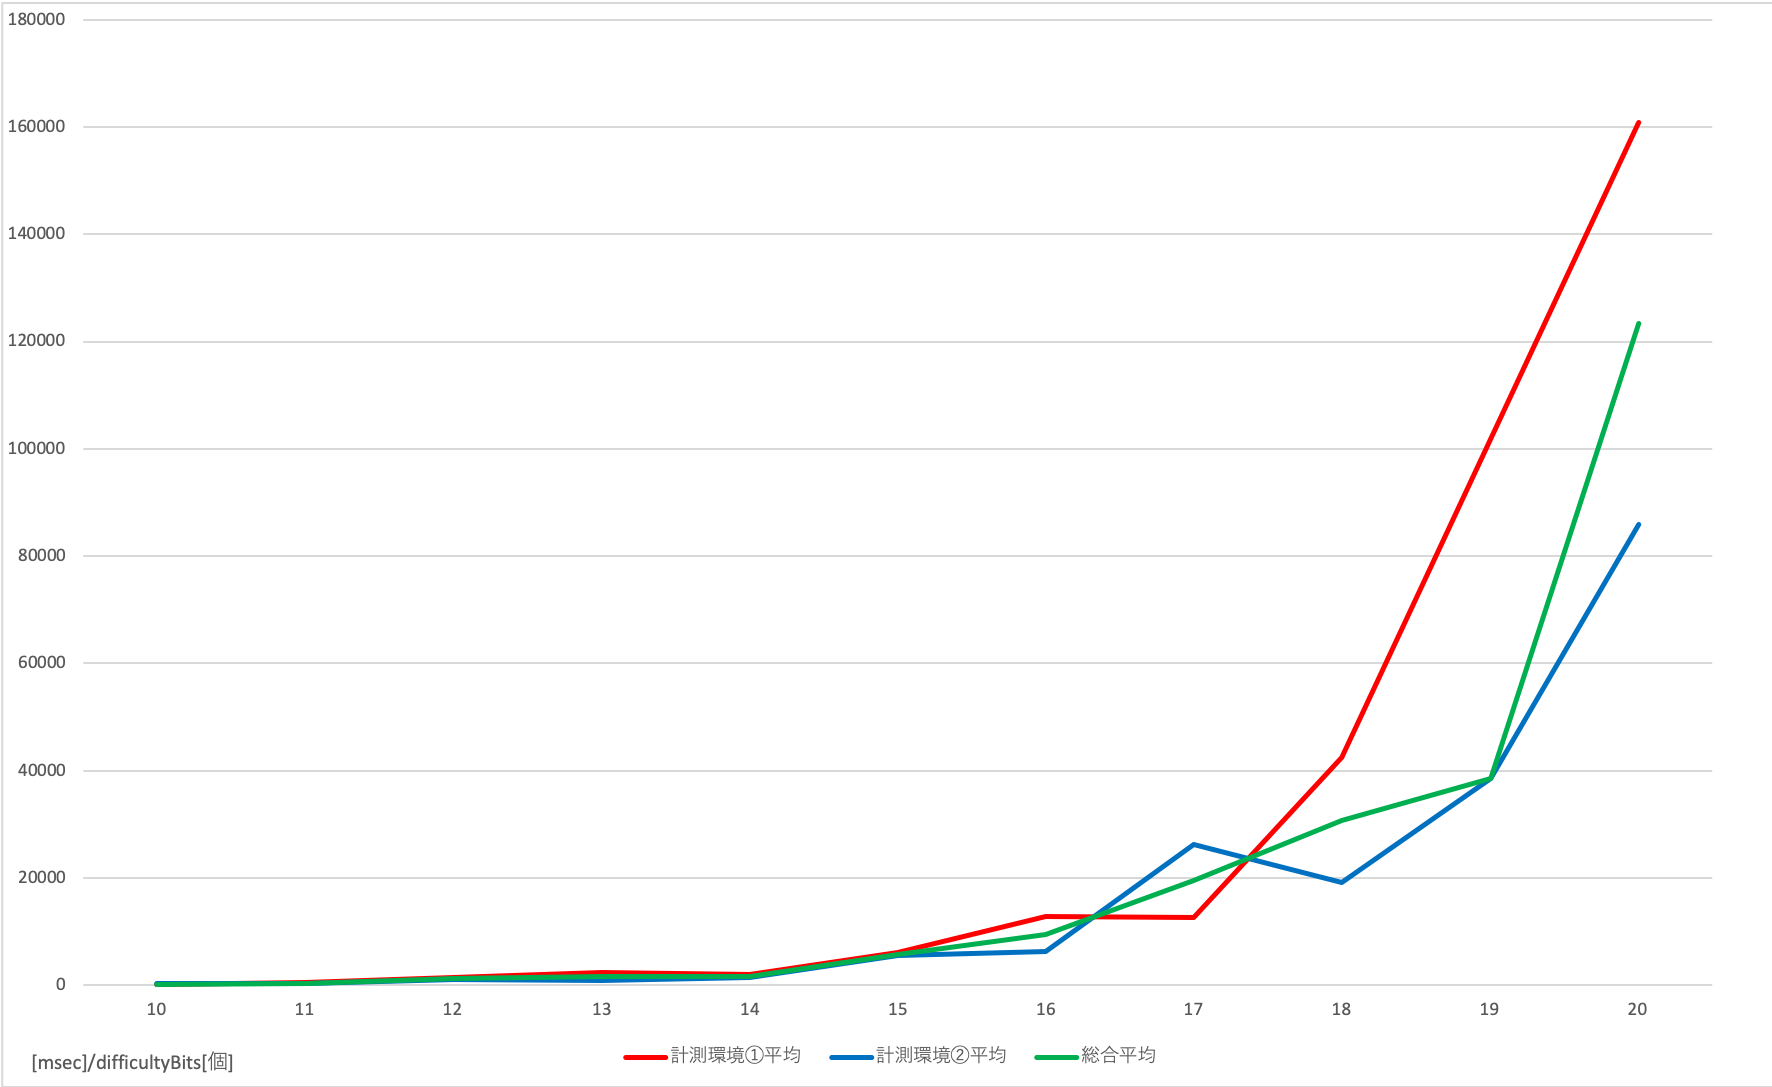
\includegraphics[width=15cm]{glaph.png}
    \caption{実行時間の変動の図}
  \end{center}
\end{figure*}

\end{document}
